\documentclass[11pt,letterpaper]{article}
\usepackage[margin=0.82in,headheight=14pt]{geometry}
\usepackage[T1]{fontenc}
\usepackage[utf8]{inputenc}
\usepackage{lmodern,amsmath,amssymb,amsthm,mathtools,microtype,booktabs,longtable,array,xcolor}
\usepackage{tikz}
\usetikzlibrary{arrows.meta,positioning,calc,fit,decorations.pathreplacing}
\usepackage{fancyhdr,hyperref,enumitem,needspace}
\hypersetup{colorlinks=true,linkcolor=black,citecolor=black,urlcolor=black,pdftitle={Portal Quotients and Decisional Memory},pdfauthor={Brian Tenneson}}
\pagestyle{fancy}\fancyhf{}\fancyhead[L]{\footnotesize Portal Quotients and Decisional Memory}\fancyhead[R]{\footnotesize Tenneson}\fancyfoot[C]{\thepage}\renewcommand{\headrulewidth}{0.3pt}
\setlength{\parskip}{3pt}\setlength{\parindent}{0pt}\setcounter{tocdepth}{1}
\setlist[itemize]{topsep=3pt,itemsep=2pt,parsep=0pt}
\newtheorem{theorem}{Theorem}[section]
\newtheorem{lemma}[theorem]{Lemma}
\newtheorem{proposition}[theorem]{Proposition}
\newtheorem{corollary}[theorem]{Corollary}
\newtheorem{definition}[theorem]{Definition}
\newtheorem{example}[theorem]{Example}
\newtheorem{remark}[theorem]{Remark}
\newcommand{\dist}{\operatorname{dist}}
\newcommand{\HH}{\mathcal H}
\newcommand{\INF}{+\infty}
\newcommand{\PP}{\mathcal P}
\newcommand{\old}{\mathrm{old}}
\newcommand{\new}{\mathrm{new}}
\newcommand{\Wzero}{\mathrm{W0}}
\newcommand{\Wone}{\mathrm{W1}}
\newcommand{\Wtwo}{\mathrm{W2}}
\newcommand{\Wthree}{\mathrm{W3}}
\newcommand{\attrib}[1]{\par\noindent\textit{Provenance and priority boundary.} #1\par}
\begin{document}
\begin{center}
{\LARGE\bfseries Portal Quotients and Decisional Memory\par}
\vspace{4pt}
{\large When Global BANK Shocks Admit Finite Boundary Representations\par}
\vspace{9pt}
{\normalsize FDWC$^3$ Level-3 Research Exposition $\cdot$ W3 $\cdot$ Version 4.1: Cited and ATLAS-Audited Edition\par}
\vspace{9pt}
{\large\textless Brian Tenneson\textgreater\par}
{\small Mathematical direction, research questions, and supervision: \textless Brian Tenneson\textgreater\par}
{\small Mathematical development and manuscript preparation assisted by OpenAI's ChatGPT\par}
{\small October 31, 2026\par}
\end{center}
\vspace{3pt}
\noindent\textbf{Source scope.} This is a new Level-3 manuscript descending from the immutable W0 (\emph{Geodesic Continuation and Multiresolution Omnicartography}), W1 (\emph{The Cost of Re-Certifying a Geodesic}), and the attached integrated W2 Version 3 (\emph{Certified Sufficiency and the Frontiers of Repair}) \cite{W0,W1,W2}. W0, W1, and W2 are not edited. The underlying W3 mathematical development used the ancestral works and their then-authorized bibliography; this separate retrospective citation edition additionally reviews relevant external scholarship for attribution and publication audit. No outside source is retroactively portrayed as a source used in the original W3 discovery. Neither the author nor the AI assistant asserts historical priority for classical shortest-path or dynamic-graph mechanisms.

\noindent\textbf{AI disclosure pointer.} The full \emph{Disclaimer on Mathematical Accuracy, Authorship, and Artificial Intelligence} is located on the \textbf{last page} of this manuscript.
\begin{abstract}
A BANK update may change the settlement distance of arbitrarily many states, while an agent still needs only a certified decision at one state. The preceding W2 investigated region-supported lower potentials and a minimal distance-ball frontier within that certificate language. This article asks a distinct question: can the effect of several added transitions be represented \emph{exactly} through a finite interface to the old geometry, without first rebuilding the new geometry? For $k$ nonnegative added edges, we construct a graph of $k$ labeled portals plus a sink whose shortest paths, together with old point-to-portal distances, exactly determine each new settlement horizon. For one edge this reduces to a scalar min-plus formula and an exact characterization of the states whose horizons change. We prove that the complete old horizon vector and the announced new edge do \emph{not} by themselves determine the updated decision: an additional old distance-to-portal coordinate can be indispensable. Certified interval versions yield sound decisions without exact portal data. Finally, an explicit family separates the \emph{support cardinality} required by W2's zero-outside frontier representation from the constant-size old-distance portal summary sufficient for the same decision. This is a separation between certificate languages under named precomputation assumptions, not a universal runtime or proof-size lower bound. The central research object is the \emph{decision-relative portal quotient}: a compact, exact account of a global change relative to a fixed query workload. All results have mathematical proofs; none has been independently machine-verified, and historical originality remains unestablished.
\end{abstract}
\tableofcontents
\section{A new question: update extent versus decisional dimension}
W0 models verifier-accepted theorem-proving transitions as a weighted graph and measures remaining work by settlement horizon. W1 distinguishes an obsolete optimality claim from an executable old route, then charges for replanning. The integrated W2 establishes a greatest cap-dominated feasible potential, zero-outside regional frontiers, and an exact distance-ball criterion for a particular no-replanning certificate \cite{W0,W1,W2}. All three emphasize how much of the updated graph must be known, repaired, or inspected.

A different mathematical quantity may matter: \emph{how many old metric measurements suffice to determine the effect of an authenticated update at the requested states?} A single new edge can alter a long chain of distances, yet its effect at a specified root may depend on only one previously certified root-to-tail distance, one old head-to-settlement distance, and the old root horizon. This motivates separating three objects:
\begin{itemize}
\item the \emph{influence set} of states whose actual horizons change;
\item the \emph{portal summary} of old distances needed to evaluate a batch of new edges;
\item the \emph{certificate language and acquisition contract} under which that summary is trustworthy.
\end{itemize}
We prove an exact representation theorem before making any claim about speed. This reversal of emphasis is deliberate: a small formula is not automatically a short certificate if the formula's old distances are expensive to establish.

\textit{Prior-art orientation (retrospective).} Shortest-path updates and min-plus path composition are established mathematical techniques \cite{Bellman,Mohri,Dynamic,Demetrescu}. Preserving information among designated terminals is also studied in graph compression, though the distance-preserving-minor problem is formally different from our fixed-edge portal quotient \cite{Krauthgamer}. Independently checkable evidence and planning/acting tradeoffs likewise have established antecedents \cite{Necula,Mugdan,Shekhar,Russell}. We claim a candidate distinctive \emph{decision-evidence formulation}, not priority for these ingredients.

\section{Finite geometry and the portal interface}
\begin{definition}[Old geometry and an authenticated edge batch]\label{def:setup}
Let $G_0=(V,E_0,w_0,\Sigma)$ be a finite directed graph with nonnegative edge weights and a nonempty settlement set $\Sigma$. Define the extended distances
\[
 d_0(u,v)=\min\{\operatorname{Len}_0(\gamma):\gamma:u\leadsto v\},\qquad
 H_0(x)=\min_{s\in\Sigma} d_0(x,s),
\]
using the value $\INF$ when no qualifying path exists. A \emph{monotone edge batch} is an authenticated set $F=\{e_i=(a_i,b_i,c_i):1\le i\le k\}$ of distinguishable new directed edges with $c_i\ge0$; old edges, costs, vertices and settlement states are unchanged. We allow labeled parallel edges as separate choices. Write $G_F=G_0\cup F$ and $H_F$ for its settlement horizon. Each added edge is accepted by the declared verifier gate; authenticity is an assumption, not an inference from its numerical weight.
\end{definition}
Nonnegative weights guarantee attainment of finite shortest paths in this finite setting. A path can be replaced by a simple path after removing nonnegative cycles without increasing its length. We do not use $\infty-\infty$, and all minima below are understood in $[0,\infty]$.

\begin{definition}[Portal graph and old-distance summary]\label{def:portal}
For each new edge $e_i$ create a portal state $i$ and create a sink $\star$. The \emph{portal graph} $\PP_F$ has edge weights
\begin{align}
 i\longrightarrow \star &: \quad h_i:=c_i+H_0(b_i),\label{eq:h}\tag{P1}\\
 i\longrightarrow j &: \quad M_{ij}:=c_i+d_0(b_i,a_j)\quad(1\le j\le k),\label{eq:M}\tag{P2}
\end{align}
where an infinite-weight option is omitted. Let $R_i=d_{\PP_F}(i,\star)$. For a query state $x$ define its \emph{portal summary}
\[
\mathcal S_F(x)=\bigl(H_0(x),\;[d_0(x,a_i)]_{i=1}^{k},\;[H_0(b_i)]_{i=1}^{k},\;[d_0(b_i,a_j)]_{i,j=1}^{k},\;[c_i]_{i=1}^{k}\bigr).
\]
The summary records $O(k^2+k)$ old distances shared by all queries, plus $k+1$ old values per query. It does not include the complete updated horizon vector.
\end{definition}
\begin{figure}[ht]
\centering
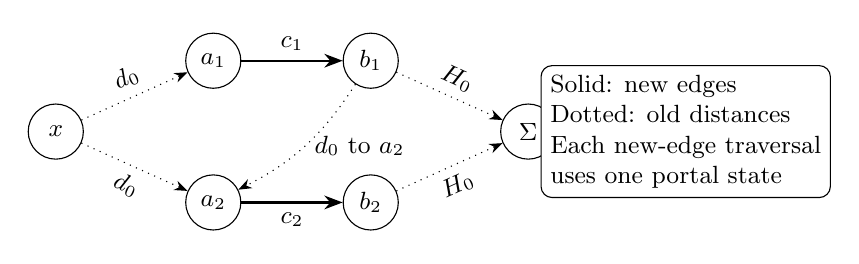
\begin{tikzpicture}[>=Stealth, node distance=16mm, every node/.style={font=\small}]
 \tikzstyle{st}=[draw,circle,minimum size=7mm,inner sep=1pt]
 \node[st] (x) at (0,0) {$x$};
 \node[st] (a1) at (2,0.9) {$a_1$}; \node[st] (b1) at (4,0.9) {$b_1$};
 \node[st] (a2) at (2,-0.9) {$a_2$}; \node[st] (b2) at (4,-0.9) {$b_2$};
 \node[st] (ss) at (6,0) {$\Sigma$};
 \draw[->,dotted] (x)-- node[above,sloped] {$d_0$} (a1);
 \draw[->,dotted] (x)-- node[below,sloped] {$d_0$} (a2);
 \draw[->,thick] (a1)-- node[above] {$c_1$} (b1);
 \draw[->,thick] (a2)-- node[below] {$c_2$} (b2);
 \draw[->,dotted] (b1)-- node[above,sloped] {$H_0$} (ss);
 \draw[->,dotted] (b2)-- node[below,sloped] {$H_0$} (ss);
 \draw[->,dotted,bend left=15] (b1) to node[right,align=center] {$d_0$ to\ $a_2$} (a2);
 \node[draw,rounded corners,align=left,fill=white] at (8.0,0) {Solid: new edges\\Dotted: old distances\\Each new-edge traversal\\uses one portal state};
\end{tikzpicture}
\caption{The portal interface: old paths become weighted macro-transitions; only actual BANK additions are drawn as solid edges. The dotted macro-transitions are numerical distances, not necessarily single graph edges.}
\label{fig:portal}
\end{figure}

\section{Exact finite-portal factorization}
\begin{theorem}[Portal quotient representation]\label{thm:portal}
Under Definition~\ref{def:setup}, for every $x\in V$,
\begin{equation}\label{eq:quotient}
\boxed{\displaystyle H_F(x)=\min\!\left\{H_0(x),\ \min_{1\le i\le k}\bigl(d_0(x,a_i)+R_i\bigr)\right\}.}
\end{equation}
Consequently the complete effect of the batch at any specified query states is determined by their portal summaries. The portal graph has $k+1$ states and at most $k^2+k$ finite arcs, irrespective of $|V|$ and irrespective of how many old paths exist.
\end{theorem}
\begin{proof}
Fix a finite-cost path $\gamma$ in $G_F$ from $x$ to $\Sigma$. If it uses no newly added edge, its cost is at least $H_0(x)$. Otherwise list its new edges in occurrence order $e_{i_1},\ldots,e_{i_m}$. The initial segment $x\leadsto a_{i_1}$ and each segment $b_{i_j}\leadsto a_{i_{j+1}}$ contain only old edges; the final segment $b_{i_m}\leadsto\Sigma$ also contains only old edges. Their lengths are at least the corresponding old distances. Thus
\[
\operatorname{Len}(\gamma)\ge d_0(x,a_{i_1})+\sum_{j<m} \bigl(c_{i_j}+d_0(b_{i_j},a_{i_{j+1}})\bigr)+c_{i_m}+H_0(b_{i_m})
\ge d_0(x,a_{i_1})+R_{i_1}.
\]
This proves the \emph{lower} inequality in \eqref{eq:quotient} after minimizing over $\gamma$. For the reverse inequality, any finite portal route $i_1,\ldots,i_m,\star$ can be expanded by choosing shortest old routes for its finite $d_0$ and $H_0$ entries and inserting $e_{i_1},\ldots,e_{i_m}$. The resulting accepted walk reaches a settlement state at cost equal to the portal expression (and may be stopped earlier if a segment passes through settlement). Similarly the old settlement path of length $H_0(x)$ remains available when finite. Therefore $H_F(x)$ is no greater than each finite candidate in \eqref{eq:quotient}. Both inequalities hold, including unreachable cases.
\end{proof}
\attrib{The path decomposition and shortest-path recurrence are classical min-plus/dynamic-programming mechanisms, anticipated in the literature already cited by W2 \cite{Bellman,Mohri,Dynamic}. Finite terminal-distance summaries and changing-edge shortest paths have direct prior-art neighborhoods \cite{Demetrescu,Krauthgamer}. The latter treats undirected distance-preserving minors, not this particular directed authenticated update construction. Our \emph{decision-evidence interpretation} is a candidate for distinctiveness relative to W0--W2; historical novelty of the factorization itself is not established.}

\begin{corollary}[Single-edge exact update]\label{cor:one}
For $F=\{(a,b,c)\}$,
\begin{equation}\label{eq:one}
\boxed{H_F(x)=\min\bigl\{H_0(x),\ d_0(x,a)+c+H_0(b)\bigr\}.}
\end{equation}
In particular the exact improvement locus is
\[
\mathcal A_F=\{x\in V:\ d_0(x,a)+c+H_0(b)<H_0(x)\}.
\]
\end{corollary}
\begin{proof}
The one-portal graph has a terminal arc of weight $c+H_0(b)$ and a nonnegative self-loop of weight $c+d_0(b,a)$. Its shortest sink distance is therefore $c+H_0(b)$, since deleting repetitions of its self-loop cannot increase the cost. Substitute in Theorem~\ref{thm:portal}. Strict comparison of the two candidates is equivalent to strict improvement in the extended-real order.
\end{proof}
\attrib{The one-edge sensitivity formula is elementary and closely related to established dynamic shortest-path updates \cite{Dynamic,Dstar,Demetrescu}. Its \emph{exact influence-set interpretation} is a manuscript-level derived consequence, not a claim of global priority.}

\begin{proposition}[Finite boundary work, conditional on old evidence]\label{prop:cost}
Assume the old distances appearing in $\mathcal S_F(x)$ for $m$ requested states are already available as authenticated and previously verified scalars. Then the new horizons at those states can be computed with $O(k^2+mk+m)$ scalar inputs and $O(k^2+mk)$ ordinary arithmetic/comparison operations using a dense nonnegative shortest-path computation on $\PP_F$. For $k=0$ take $H_F=H_0$. Neither the original acquisition cost nor storage/verification cost of those old certificates is bounded by this claim.
\end{proposition}
\begin{proof}
The portal graph has $k+1$ vertices and at most $k^2+k$ arcs. A direct dense implementation of Dijkstra's algorithm finds all $R_i$ from the sink in its reverse graph in $O(k^2)$ comparisons and additions. Formula \eqref{eq:quotient} takes $O(k)$ comparisons per root, hence $O(mk)$. The displayed scalar count includes the shared $k^2$ old head-to-tail distances and the query-specific $mk$ distances. There is no operation on unrequested new horizons. The statement presupposes the old scalar witnesses rather than supplying them for free.
\end{proof}
\attrib{Algorithmic operations are established shortest-path operations \cite{Dijkstra,Dynamic,Demetrescu}; the parameterized portal-input accounting is a new \emph{relative-to-ancestry} formulation, not a lower bound against arbitrary data structures.}

\section{Why the old horizon vector is not enough}
\begin{theorem}[Horizon-only nonidentifiability]\label{thm:inadequate}
There exist two finite nonnegative old graphs on the same labeled vertices, with identical complete old settlement-horizon vectors and identical announced new edge, for which the new horizon at the same root differs. Moreover, for a fixed accepted old route and a fixed positive replanning charge, an idealized go-versus-replan decision can have opposite outcomes in the two updated graphs.
\end{theorem}
\begin{proof}
Use vertices $x,a,b,t$ and settlement set $\{t\}$. In each old graph place edges $x\to t$ of cost $10$, $a\to t$ of cost $20$, $b\to t$ of cost $0$, and $x\to a$ of cost $\lambda$. Take $\lambda=1$ in the first graph and $\lambda=11$ in the second. Both old horizon vectors are identical:
\[
H_0(x)=10,\qquad H_0(a)=20,\qquad H_0(b)=H_0(t)=0,
\]
because the route via $a$ initially costs at least $21$. In each graph add exactly the same authenticated edge $a\to b$ of weight $0$. Formula \eqref{eq:one} gives $H_F(x)=\min\{10,\lambda\}$, hence $H_F(x)=1$ and $10$, respectively. Take the retained accepted route $x\to t$ of cost $P=10$, and an ideal replan-first stage of compulsory cost $c=2$ that can subsequently execute a new shortest path. In the first instance it completes in $2+1=3<10$, so Go loses. In the second it completes in $2+10=12>10$, so Go wins. An observer provided only the old horizon vector and the new-edge announcement sees identical inputs and cannot determine the correct outcome in both cases. The missing distinguishing scalar is $d_0(x,a)=\lambda$.
\end{proof}
\attrib{The adversarial indistinguishability technique is standard; dynamic-distance algorithms already distinguish old distance data from post-update distances \cite{Dynamic,Demetrescu}. The particular \emph{horizon-vector/decision} counterexample is developed here and is a candidate for distinctiveness as an application, not as a new lower-bound method. A complete old graph, unlike merely its horizon vector, would distinguish the two instances.}

\begin{figure}[ht]
\centering
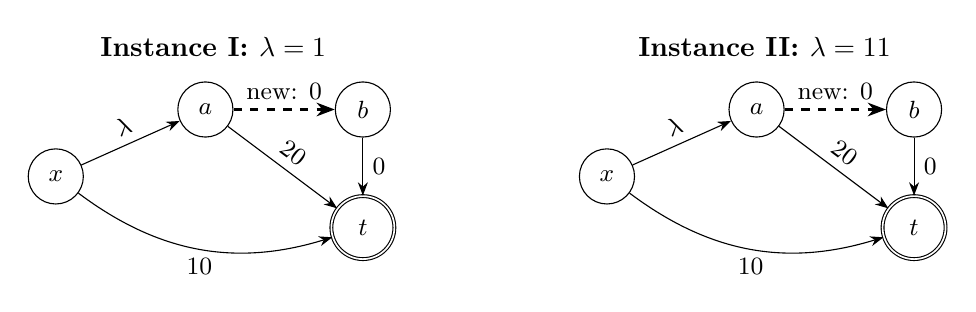
\begin{tikzpicture}[>=Stealth, every node/.style={font=\small}]
\foreach \dx/\val/\lbl in {0/1/Instance I,7/11/Instance II}{
 \node[font=\bfseries] at (\dx+2,1.65) {\lbl: $\lambda=\val$};
 \node[draw,circle,minimum size=7mm] (x\dx) at (\dx+0,0) {$x$};
 \node[draw,circle,minimum size=7mm] (a\dx) at (\dx+1.9,0.85) {$a$};
 \node[draw,circle,minimum size=7mm] (b\dx) at (\dx+3.9,0.85) {$b$};
 \node[draw,double,circle,minimum size=8mm] (t\dx) at (\dx+3.9,-0.65) {$t$};
 \draw[->] (x\dx) -- node[above,sloped] {$\lambda$} (a\dx);
 \draw[->,thick,dashed] (a\dx) -- node[above] {new: $0$} (b\dx);
 \draw[->] (b\dx) -- node[right] {$0$} (t\dx);
 \draw[->] (a\dx) -- node[above,sloped] {$20$} (t\dx);
 \draw[->,bend right=27] (x\dx) to node[below] {$10$} (t\dx);
}
\end{tikzpicture}
\caption{Two graphs with the same old complete horizon map and the same new edge, but different root-to-portal distance and opposite idealized decisions for $P=10,c=2$. Dashed edges are newly approved.}
\end{figure}

\begin{remark}[Summary adequacy is query-relative]
Agreeing on all entries of a portal summary forces agreement on the corresponding updated root horizon by Theorem~\ref{thm:portal}. The converse is false: distinct summaries can produce the same minimum. Thus $\mathcal S_F(x)$ is a \emph{sufficient statistic} for a chosen query, not automatically a minimal description of its answer. Theorem~\ref{thm:inadequate} proves only that a particular omitted coordinate can matter, not that every entry is indispensable for every input.
\end{remark}

\section{Certificate-bearing approximate portal quotients}
\begin{proposition}[Checking old metric coordinates]\label{prop:metricverify}
For a finite old graph with nonnegative rational weights and authenticated complete outgoing records, a claimed finite value $d_0(u,v)=D$ can be checked from (i) an old legal $u$-to-$v$ path of cost $D$, and (ii) an authenticated feasible lower potential $q:V\to\mathbb Q_{\ge0}$ with $q(v)=0$, $q(z)\le w_0(z,z')+q(z')$ on every old edge, and $q(u)=D$. The corresponding settlement-distance claim $H_0(u)=D$ is checked by a path ending in $\Sigma$ and a feasible $q$ vanishing on all settlements. An infinite point-to-point distance can instead be certified by a set containing $u$ and excluding $v$, closed under all old outgoing transitions. These witnesses can be large; their existence does not imply constant proof size or constant verifier work.
\end{proposition}
\begin{proof}
The path establishes $d_0(u,v)\le D$. Summing feasible inequalities over any path from $u$ to $v$ yields $q(u)\le\operatorname{Len}(\gamma)+q(v)=\operatorname{Len}(\gamma)$, so $d_0(u,v)\ge D$. Replacing $v$ by the settlement set gives the analogous argument for $H_0$. If a set $U$ contains $u$, excludes $v$, and every outgoing edge from $U$ stays in $U$, any path beginning at $u$ stays in $U$ and cannot reach $v$. For an unreachable pair, the actual forward-reachable set from $u$ is such a set; checking its closure requires the declared complete outgoing records.
\end{proof}
\attrib{Graph potentials and path witnesses are established lower/upper-bound certificates; independent certificate checking has close predecessors in proof-carrying code and optimal classical planning \cite{W1,W2,Necula,Mugdan}. The proposition explicitly states how the old distance data assumed by the portal quotient can be authenticated; it adds no new complexity claim.}
Exact old point-to-point distances may be expensive or unavailable. The portal quotient also has a one-sided, independently checkable version, which is what makes it relevant to verifier-gated agents rather than to graph algebra alone.
\begin{definition}[Certified portal intervals]
For every distance used in $\mathcal S_F(x)$, suppose the checker has a sound interval $\underline d_0\le d_0\le\overline d_0$ or $\underline H_0\le H_0\le\overline H_0$, allowing $\INF$. The added-edge weights $c_i$ are exact and authenticated. Form lower and upper portal graphs by substituting the respective endpoints of the intervals in \eqref{eq:h}--\eqref{eq:M}; write $\underline R_i,\overline R_i$ for their sink distances, and define
\begin{align*}
\underline H_F(x)&=\min\bigl\{\underline H_0(x),\ \min_i(\underline d_0(x,a_i)+\underline R_i)\bigr\},\\
\overline H_F(x)&=\min\bigl\{\overline H_0(x),\ \min_i(\overline d_0(x,a_i)+\overline R_i)\bigr\}.
\end{align*}
The intervals must be \emph{certified} under an explicit trust model: numbers merely reported by an oracle are not certificates.
\end{definition}
\begin{theorem}[Sound interval portal representation]\label{thm:interval}
For every query state with sound input intervals,
\[
\boxed{\underline H_F(x)\le H_F(x)\le\overline H_F(x).}
\]
The lower and upper portal bounds are monotone in the input bounds. In particular refining all intervals cannot decrease $\underline H_F(x)$ or increase $\overline H_F(x)$.
\end{theorem}
\begin{proof}
The length of every fixed portal route is a sum of nonnegative inputs. Replacing every input by a pointwise lower (respectively upper) bound decreases (respectively increases) that route's total, with extended sums interpreted conventionally. Taking a minimum over the same finite combinatorial paths preserves the order; simple routes suffice because weights are nonnegative. Apply the same monotonicity to the outer minimum in \eqref{eq:quotient}. Nested interval refinement applies this order twice, proving the final assertion.
\end{proof}
\attrib{The monotonicity of min-plus expressions is established mathematics \cite{Mohri,Bellman}. The use of authenticated old metric intervals to bound a \emph{batch-updated decision} is a derived W3 interface, potentially distinctive as a combination but not as an inequality.}

\begin{corollary}[Portal-certified stopping without global repair]\label{cor:stop}
Let $\pi$ be a verifier-accepted complete settlement route that remains executable after the batch, with known post-update cost $P$. In a static one-decision model, suppose a replanning-first policy must spend a compulsory sequential nonoverlapping time $c>0$ before executing any settlement route, with edge weights equal to execution-and-verification time. If
\[
\boxed{c>P-\underline H_F(x),}
\]
then executing $\pi$ immediately finishes strictly sooner than every such replan-first policy. Conversely, failure of this sufficient inequality does not authorize replanning.
\end{corollary}
\begin{proof}
Immediate execution takes $P$. Every replan-first policy takes at least $c+H_F(x)\ge c+\underline H_F(x)>P$. If the inequality fails, the available lower evidence may simply be weak; no comparison in the other direction follows.
\end{proof}
\attrib{The stopping comparison is inherited from W1 and W2 and has longstanding planning-versus-execution antecedents \cite{W1,W2,Shekhar,Russell}; the new part is that the \emph{lower input} comes from the W3 portal quotient rather than a zero-outside regional frontier. Not claimed as a historically new metareasoning principle.}

\begin{proposition}[Root and outgoing-edge decision equivalence]\label{prop:actions}
Suppose the verifier has sound portal intervals for $H_F(y)$ at the head $y$ of \emph{every legal outgoing edge} of a fixed nonterminal state $x$, including newly added and labeled parallel edges, and exact post-update first-edge costs. If one labeled edge $e=(x,a)$ satisfies
\[
 w_F(e)+\overline H_F(a)<w_F(f)+\underline H_F(z_f)
 \quad\text{for every other legal outgoing edge }f=(x,z_f),
\]
then $e$ is the uniquely minimum-cost first edge in the updated graph. With exact portal summaries this strict interval criterion is also necessary for a uniquely minimum-cost outgoing edge, provided all outgoing edges are included. Geodesic continuation additionally requires a reachable settlement and the usual path-attainment hypotheses.
\end{proposition}
\begin{proof}
The true continuation cost of $e$ is no greater than its certified upper endpoint, while that of each different edge $f$ is no less than its certified lower endpoint. Hence the inequalities give strict minimum cost over all legal outgoing \emph{edges}, including edges with the same head. With exact inputs both bounds equal the corresponding true horizon by Theorem~\ref{thm:portal}; strict unique minimum cost is then equivalent to the displayed inequalities. For a nonterminal root with finite horizon, shortest-path attainment identifies the minimum-cost first edge with geodesic continuation.
\end{proof}
\attrib{The interval-separation comparison is inherited from W0 and W2 \cite{W0,W2,Hart,Mugdan}; only the source of the interval evidence changes here. This edition repairs the original successor-vertex wording to compare all \emph{labeled outgoing edges}, so parallel-edge ties are not silently omitted.}

\section{A strict separation between certificate languages}
W2's integrated Version 3 proves that, for a cap $b$, a zero-outside inspected region $K$, and $p_K=\operatorname{cl}_{G_F}(b\mathbf1_K)$,
\begin{equation}\label{eq:w2}
p_K(x)=\min\bigl\{p_V(x),\ d_{G_F}(x,V\setminus K)\bigr\}.
\end{equation}
It consequently identifies a unique inclusion-minimal \emph{region} for a specified stopping threshold within this language \cite[Theorems 5.2 and 6.4]{W2}. This is not a claim of minimality across all mathematically valid certificate encodings. The portal quotient reveals a rigorous disparity.

\begin{theorem}[Global shock, growing regional support, fixed portal width]\label{thm:separate}
For every integer $n\ge4$ there is an $n+2$ vertex monotone one-edge update with all finite old horizons such that:
\begin{enumerate}[label=(\roman*)]
\item the update strictly changes the settlement horizon of all $n$ nonsettlement states;
\item for a fixed accepted route $P=n$ and compulsory replanning charge $c=3/2$, the W2 zero-outside frontier stopping test using cap $b=H_0$ has a unique inclusion-minimal passing region with exactly $n-1$ vertices;
\item a preauthenticated single-edge portal summary of three old scalar distances/values, together with the new edge and retained route, determines the exact updated root horizon and certifies the same stopping decision.
\end{enumerate}
This is a separation between \emph{support cardinality in one certificate language} and \emph{scalar summary width in another}, assuming the old scalar certificates are available. It is not a post-update query lower bound against arbitrary caching or a bound on total proof bits.
\end{theorem}
\begin{proof}
Take vertices $v_0,\ldots,v_{n-1},t,s$ and settlements $\Sigma=\{t,s\}$. The old graph contains the chain
\[
v_0\xrightarrow{1}v_1\xrightarrow{1}\cdots\xrightarrow{1}v_{n-1}\xrightarrow{1}t,
\]
with $s$ isolated. Let $x=v_0$, $a=v_{n-1}$, and add the single authenticated edge $a\xrightarrow{0}s$. For $0\le i<n$,
\[
H_0(v_i)=n-i,\qquad H_F(v_i)=n-1-i.
\]
Thus all $n$ nonsettlement states change. Retain the complete old path $x\leadsto t$ of cost $P=n$, and take $c=3/2$. The updated horizon is $H_F(x)=n-1$, so $c>P-H_F(x)=1$ and immediate execution is the winning certified choice.

For the W2 frontier, the cap is $b=H_0$. Its global closure under the one-edge update is $p_V=H_F$ by the inherited exact-cap-repair result. Set $T=P-c=n-3/2$. W2's exact distance-ball characterization says the zero-outside test passes precisely when $K$ includes every vertex of $G_F$ at distance at most $T$ from $x$. These are exactly $v_0,\ldots,v_{n-2}$: $d_{G_F}(x,v_i)=i$, while $d_{G_F}(x,v_{n-1})=n-1>T$, $d_{G_F}(x,s)=n-1>T$, and $d_{G_F}(x,t)=n>T$. Hence the unique minimal passing region contains $n-1$ vertices.

For the portal calculation, the three old scalars are $H_0(x)=n$, $d_0(x,a)=n-1$, and $H_0(s)=0$. The authenticated new edge has cost zero. Corollary~\ref{cor:one} returns $H_F(x)=\min\{n,n-1+0+0\}=n-1$. The inequality $3/2>n-(n-1)=1$ proves the same stopping decision. These scalar claims are assumed previously authenticated, and the old path certificate retained; their historical construction is not charged at zero.
\end{proof}
\attrib{The growing-region ball is inherited from W2; the chain is elementary. Distance preservation under selected terminal summaries and dynamic shortest paths have extensive antecedents \cite{W2,Krauthgamer,Demetrescu}. The contrast between \emph{zero-outside support cardinality and preauthenticated portal-coordinate width} is a candidate distinctive comparison relative to ancestry, not a proof-size, verification-time, or unrestricted data-structure separation.}

\begin{figure}[ht]
\centering
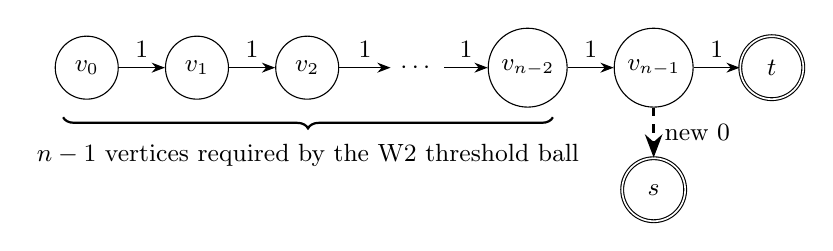
\begin{tikzpicture}[>=Stealth, every node/.style={font=\small}]
\node[draw,circle,minimum size=8mm] (v0) at (0,0) {$v_0$};
\node[draw,circle,minimum size=8mm] (v1) at (1.4,0) {$v_1$};
\node[draw,circle,minimum size=8mm] (v2) at (2.8,0) {$v_2$};
\node (dots) at (4.2,0) {$\cdots$};
\node[draw,circle,minimum size=8mm] (vlastm) at (5.6,0) {$v_{n-2}$};
\node[draw,circle,minimum size=8mm] (vlast) at (7.2,0) {$v_{n-1}$};
\node[draw,double,circle,minimum size=8mm] (t) at (8.7,0) {$t$};
\node[draw,double,circle,minimum size=8mm] (s) at (7.2,-1.55) {$s$};
\draw[->] (v0)-- node[above] {$1$} (v1);
\draw[->] (v1)-- node[above] {$1$} (v2);
\draw[->] (v2)-- node[above] {$1$} (dots);
\draw[->] (dots)-- node[above] {$1$} (vlastm);
\draw[->] (vlastm)-- node[above] {$1$} (vlast);
\draw[->] (vlast)-- node[above] {$1$} (t);
\draw[->,very thick,dashed] (vlast)--node[right] {new $0$}(s);
\draw[decorate,decoration={brace,mirror,amplitude=4pt},thick] (-0.3,-0.63)-- (5.92,-0.63) node[midway,below=6pt] {$n-1$ vertices required by the W2 threshold ball};
\end{tikzpicture}
\caption{All $n$ nonterminal horizons improve, and the W2 zero-outside frontier needs $n-1$ supported vertices for this threshold; an already certified one-edge portal summary uses three old numbers. The dashed arrow is the only added edge.}
\end{figure}

\section{Composition, obstructions, and interpretation}
\begin{proposition}[Batch-order invariance without a free update algorithm]\label{prop:batch}
For two authenticated nonnegative new-edge batches $F$ and $J$ on the same old graph, the exact horizon obtained by applying $F$ then $J$ equals the horizon obtained by applying $J$ then $F$, and both agree with the portal formula for $F\cup J$. However, the old-distance portal summaries for the two batches generally do not suffice \emph{separately} to compute the union result without the cross-distances $d_0(b_i,a_j)$ linking edges of opposite batches.
\end{proposition}
\begin{proof}
The final graph is $G_0\cup F\cup J$ regardless of insertion order, so its path infimum is order-independent. Theorem~\ref{thm:portal} therefore applies to the union. For the final assertion, paths may use an edge from $F$, an old path to the tail of an edge from $J$, and then that new edge; their costs explicitly include old distances between heads in one batch and tails in the other, precisely the cross-batch portal weights. Such data are not contained in two isolated summary matrices unless separately supplied. For a concrete witness, use old vertices $x,a,b,c,d,t$, with old edges $x\to a$ of weight zero, $b\to c$ of weight $q>0$, $d\to t$ of weight zero, and no other settlement paths from $x$; add $F=\{a\to b\}$ and $J=\{c\to d\}$ of weight zero. The union horizon at $x$ is $q$, which changes with the cross-distance $d_0(b,c)=q$, while the within-batch portal data remain at infinite values and the initial old settlement horizon at $x$ is infinite.
\end{proof}
\attrib{Set-union invariance is elementary, and cross-batch distances arise from concatenating paths through distinct updates \cite{Bellman,Mohri,Dynamic,Demetrescu}. This limits effortless amortization under repeated deposits and is not a claim to a historically novel dynamic-graph theorem.}

\begin{remark}[The three irreducible accounting questions]
The formal theory separates (a) \emph{algebraic width}: how many old distance values enter the quotient; (b) \emph{evidential weight}: how much data must be authenticated to justify those values; and (c) \emph{operational latency}: whether paying to acquire or refine evidence is worth it. Theorem~\ref{thm:separate} separates (a) from W2's region size, but does not establish an advantage in (b) or (c) without a priced acquisition model. This distinction is essential to an honest originality and performance claim.
\end{remark}

\begin{remark}[Scope of the edge-update restriction]
A decrease in the weight of an old edge can be modeled as an additional distinguishably labeled parallel edge of the smaller cost, preserving the old alternative; the portal theorem then applies to the enlarged multigraph. Edge deletions, weight increases without retained old options, changes to the settlement policy, and creation of new vertices with uncertified state semantics require a new model and are not covered by the stated monotone theorem. Informal oracle recommendations cannot substitute for authenticated macro-distance certificates.
\end{remark}

\section{Further mathematical questions}
The results suggest several problems that are distinct from simply computing additional W2 frontiers.
\begin{enumerate}[label=Q\arabic*.]
\item \textbf{Minimal sufficient portal coordinates.} For a fixed update and a fixed finite workload, characterize the smallest collection of old-distance coordinates from which the action predicate can be reconstructed across an explicitly declared family of possible old graphs. Theorem~\ref{thm:inadequate} proves one necessity example, not a general optimal characterization.
\item \textbf{Proof-carrying portal compression.} What is the exact cost, in proof size and verifier work, of authenticating $d_0(b_i,a_j)$ and $d_0(x,a_i)$, including unreachable-pair claims? Determine graph families where a compact shared witness exists and where any such witness must be large under a fixed proof language.
\item \textbf{Online BANK batches.} Under repeated updates with no free precomputation, compare the amortized cost of maintaining the portal quotient with incremental shortest-path methods. Cross-batch distances prevent naive independent composition.
\item \textbf{From toy graphs to theorem-prover states.} Establish explicit, checkable conditions under which a real ATP's successor relation and BANK changes admit complete closed-world authenticated records and usable cached metric certificates. Without these conditions the portal representation remains a finite formal model.
\end{enumerate}

\section{Conclusion}
The influence of a new verified transition and the information required to assess that influence are different mathematical objects. W2 showed that a single update can produce a large affected region, and identified a unique threshold ball within a specified regional-certificate language. W3 replaces the size of that region as its central organizing question with \emph{decision-relative information}. A batch of $k$ added edges has an exact $(k+1)$-state portal quotient over old distances; one added edge may affect every predecessor in a long chain, yet a root horizon can depend on three preverified scalar values. Conversely, knowing the entire old horizon vector is not sufficient without certain point-to-portal data. This pairing---global change with compact conditional sufficiency, and global memory with decisional insufficiency---is the mathematical identity of the present exposition.

The results are exact within their finite, nonnegative, authenticated model. They do not imply that the old distance proofs were cheap, that every BANK has small portal width, that an actual theorem prover offers closed-world successor access, or that the proposed representation is historically novel.

\appendix
\section{Level-3 research, comparison, provenance and verification ledger}
\subsection*{Ancestral dependence and genuine departures}
\textbf{W0.} Verifier-gated Pioneer state geometry, settlement horizons, geodesic continuation, and BANK monotonicity \cite{W0}. \textbf{W1.} Accepted-route portability, feasibility of lower potentials, and the compulsory-delay no-replanning criterion \cite{W1}. \textbf{W2 (attached Version 3).} Capped min-plus repair, zero-outside frontier potentials, threshold distance-ball minimality, and an output-format-specific local/global separation \cite{W2}. \textbf{W3.} The portal quotient for batched edge additions, exact single-edge influence formula, horizon-vector insufficiency counterexample, portal interval stopping certificates, and a separation between \emph{certificate languages}, rather than between a local certificate and explicit whole-map output.

\subsection*{Distinct Level-3 research directions considered}
\begin{center}\small
\begin{tabular}{@{}p{0.14\linewidth}p{0.37\linewidth}p{0.39\linewidth}@{}}\toprule
Internal line & Mathematical opportunity & Comparison and disposition\\\midrule
A: Portal algebra & Decompose updated paths into old metric segments and new verified edges; obtain exact quotient and counterexamples. & Strongest complete representation theorem, concrete claims, and independent central problem; chosen.\\
B: Evidence alternatives & Model possible completions and records that distinguish counterfactual decisions. & Promising information-obstruction formulation, but stronger minimality/complexity claims require a carefully delimited hypothesis and query model; not asserted here.\\
C: Repeated decisions & Price incremental acquisition and reuse under multiple BANK deposits. & Could yield amortized bounds; cross-batch metric dependencies prevent a free composition theorem. Preserved as an open problem, not hidden.\\\bottomrule
\end{tabular}
\end{center}
Rubric: correctness and explicit quantifiers (A strong; B/C require more model choices), mathematical depth (A gives exact factorization and limitations), independence from W2 (A changes the measured object from regions to summaries), originality relative to ancestry (A adds an absent representation and two separations), explanatory coherence (A focuses on one portal geometry), further potential (A opens certificate-size questions), and dependence on inherited results (all lines depend on finite shortest paths; A does not inherit W2's zero-outside restriction). No numerical merit scores or global superiority claims are inferred.

\subsection*{Claim-level originality and responsibility table}
\small
\begin{longtable}{@{}p{0.22\linewidth}p{0.38\linewidth}p{0.31\linewidth}@{}}
\toprule
W3 claim & Nearest antecedent & Status relative to W0--W2; priority limit\\\midrule\endhead
Theorem~\ref{thm:portal} & Classical min-plus paths and dynamic shortest paths \cite{Mohri,Dynamic,Demetrescu}; W2 & New to the supplied chain as a portal representation; \emph{candidate distinctive formulation}, not demonstrated historical novelty.\\
Corollary~\ref{cor:one} & Dynamic shortest-path edge sensitivity \cite{Dynamic,Demetrescu} & Derived special case; mechanism likely classical.\\
Proposition~\ref{prop:cost} & Classical Dijkstra computation \cite{Dijkstra} & Derived conditional accounting; certificate setup costs excluded.\\
Theorem~\ref{thm:inadequate} & Dynamic shortest paths \cite{Dynamic}; W2 local-view obstruction & New counterexample for \emph{horizon-only} decisional insufficiency relative to ancestry; candidate distinctive application.\\
Proposition~\ref{prop:metricverify} & Path witnesses and feasible potentials \cite{Necula,Mugdan,W1} & Established certificate pairing, inherited from W1/W2; may require global checking.\\
Theorem~\ref{thm:interval} & Min-plus monotonicity \cite{Mohri} and W2 bounds & Derived interval representation; established algebra, new interface.\\
Corollary~\ref{cor:stop} & Planning/execution costs \cite{Shekhar,Russell}; W1/W2 & Inherited principle with portal-bounded input.\\
Proposition~\ref{prop:actions} & Heuristic bound separation \cite{Hart,W0,W2} & Inherited rule instantiated on portal intervals.\\
Theorem~\ref{thm:separate} & W2 threshold ball; terminal metrics \cite{Krauthgamer} & Candidate-original \emph{relative certificate-language separation}; no total-cost complexity claim.\\
Proposition~\ref{prop:batch} & Dynamic paths and min-plus closure \cite{Dynamic,Mohri} & Derived order independence and cross-batch information obstruction.\\\bottomrule
\end{longtable}
\normalsize
\subsection*{Version 4.1 retrospective attribution audit}
This edition compares all ten named results with their nearest known antecedents and labels each as an established mechanism, a derived specialization, or a candidate distinctive formulation. A citation points to the relevant mathematical tradition or source; it does \emph{not} imply an exact published theorem match unless explicitly stated. The portal formula is a finite path-composition identity and its mathematical novelty has not been established. The promising work-specific candidates are (i) the horizon-vector/decision counterexample as an interface distinction, and (ii) the explicit comparison between frontier-region support and preauthenticated portal-coordinate width. Neither is an unconditional proof-size or asymptotic speedup theorem. A proof-relevant editorial repair replaces successor-vertex comparisons in Proposition~\ref{prop:actions} with comparisons over all labeled outgoing edges, including parallel edges. No independent proof assistant or referee has checked this edition.

\subsection*{Audit results and outstanding obligations}
The mathematical statements were checked for terminal-path conventions, extended distances, nonnegative cycles, absence of old settlement reachability, missing old distance certificates, newly introduced first moves, strictness at a replanning threshold, and the possibility of negative edge updates (excluded). A portal-walk expansion is valid because each finite macro-distance is realized by an old path. The $n$-chain separation counts supported \emph{vertices}, not inspected records or total proof bytes. The nonidentifiability example retains identical old horizons across all vertices. No external theorem prover, independently running AMLD+++0, formal proof assistant, or third-party reviewer verified these proofs. No exhaustive originality or literature search was performed for W3, and no empirical ATP performance advantage is asserted. The W0--W2 files are unchanged.

\section*{References and retrospective scholarly context}
\addcontentsline{toc}{section}{References and retrospective scholarly context}
\begin{thebibliography}{99}\small
\bibitem{W0} \textless Brian Tenneson\textgreater, \emph{Geodesic Continuation and Multiresolution Omnicartography: Pioneers, Directional Gaps, Advance Certification, and Oracle Guidance in AMLDs}, Version 4, October 31, 2026. Ancestral source W0.
\bibitem{W1} \textless Brian Tenneson\textgreater, \emph{The Cost of Re-Certifying a Geodesic: Portable Evidence, BANK Shocks, and Decision Latency in Multiresolution Omnicartography}, FDWC Level-1 multiarticle, Version 2, October 31, 2026. Source W1.
\bibitem{W2} \textless Brian Tenneson\textgreater, \emph{Certified Sufficiency and the Frontiers of Repair: Local Proof Evidence, Nonlocal BANK Shocks, and a Conditional Work Separation}, integrated FDWC$^2$ research exposition, Version 3, October 31, 2026. Directly supplied source W2.
\bibitem{Bellman} R. Bellman, ``On a Routing Problem,'' \emph{Quarterly of Applied Mathematics} 16 (1958), 87--90. Listed in W2's bibliography.
\bibitem{Dijkstra} E. W. Dijkstra, ``A Note on Two Problems in Connexion with Graphs,'' \emph{Numerische Mathematik} 1 (1959), 269--271. Listed in W2's bibliography.
\bibitem{Hart} P. E. Hart, N. J. Nilsson, and B. Raphael, ``A Formal Basis for the Heuristic Determination of Minimum Cost Paths,'' \emph{IEEE Transactions on Systems Science and Cybernetics} 4(2) (1968), 100--107. Listed in W2's bibliography.
\bibitem{Russell} S. Russell and E. Wefald, ``Principles of Metareasoning,'' \emph{Artificial Intelligence} 49 (1991), 361--395. Listed in W2's bibliography.
\bibitem{Dynamic} G. Ramalingam and T. Reps, ``An Incremental Algorithm for a Generalization of the Shortest-Path Problem,'' \emph{Journal of Algorithms} 21(2) (1996), 267--305. Listed in W2's bibliography.
\bibitem{Mohri} M. Mohri, ``Semiring Frameworks and Algorithms for Shortest-Distance Problems,'' \emph{Journal of Automata, Languages and Combinatorics} 7(3) (2002), 321--350. Listed in W2's bibliography.
\bibitem{Dstar} S. Koenig, M. Likhachev, and D. Furcy, ``Lifelong Planning A*,'' \emph{Artificial Intelligence} 155 (2004), 93--146. Listed in W2's bibliography.

\bibitem{Shekhar} S. Shekhar and S. Dutta, ``Minimizing Response Times in Real Time Planning and Search,'' \emph{Proceedings of IJCAI-89} (1989), 238--241. \url{https://ijcai.org/proceedings/1989/38}.
\bibitem{Necula} G. C. Necula, ``Proof-Carrying Code,'' \emph{Proceedings of POPL '97} (1997), 106--119. doi:10.1145/263699.263712.
\bibitem{Demetrescu} C. Demetrescu and G. F. Italiano, ``Fully Dynamic All Pairs Shortest Paths with Real Edge Weights,'' \emph{Journal of Computer and System Sciences} 72(5) (2006), 813--837. doi:10.1016/j.jcss.2005.05.005.
\bibitem{Krauthgamer} R. Krauthgamer, H. L. Nguyen, and T. Zondiner, ``Preserving Terminal Distances Using Minors,'' \emph{SIAM Journal on Discrete Mathematics} 28(1) (2014), 127--141. doi:10.1137/120888843. Note: undirected graph minors are not identical to the directed portal construction here.
\bibitem{Mugdan} E. Mugdan, R. Christen, and S. Eriksson, ``Optimality Certificates for Classical Planning,'' \emph{Proceedings of ICAPS} 33(1) (2023), 286--294. doi:10.1609/icaps.v33i1.27206.

\end{thebibliography}
\noindent\textit{Literature scope.} The references preceding Shekhar, Necula, Demetrescu, Krauthgamer, and Mugdan were carried from W2; the five additional references were consulted retrospectively for this Version 4.1 publication review, using accessible scholarly or publisher records. This selective review is not an exhaustive historical novelty search. The result table distinguishes \emph{new relative to the manuscript ancestry} from \emph{historically original}. The latter is not established.

\clearpage
\section*{Disclaimer on Mathematical Accuracy, Authorship, and Artificial Intelligence}
\addcontentsline{toc}{section}{Disclaimer on Mathematical Accuracy, Authorship, and Artificial Intelligence}
\noindent Every reasonable effort has been made to prepare a mathematically defensible exposition with explicit definitions, valid arguments, honest hypotheses, appropriate counterexamples, and faithful attribution. ``Complete'' refers here to the coverage of pertinent stated facts or, when explicitly specified, a finite numeric object; it does not mean completeness in G\"odel's technical sense. Neither correctness, logical consistency, provability, factual completeness, nor historical originality is guaranteed. Results are intended to follow from their stated assumptions but have not been independently machine-verified, peer reviewed, or experimentally validated in a deployed automated theorem prover.

This manuscript is a hybrid human--AI work. Mathematical seeds, research directions, oversight, editorial choices, and publication decisions are attributed to \textless Brian Tenneson\textgreater. OpenAI's ChatGPT contributed definitions, proof development, examples, counterexamples, organization, text, and character-level composition; its contribution is substantial but not exclusive authorship. The labels FDWC$^3$, forward research writer, backward scout, and internal candidates describe a mathematical drafting and scrutiny procedure, not independently observed software agents or independent automated verification. The historical source chain W0 $\to$ W1 $\to$ W2 $\to$ W3 is explicitly recorded; the prior manuscripts are not altered. Several references outside W0--W2 were inherited from W2's bibliography; five further scholarly references were consulted retrospectively for attribution and this audit edition, not for the original W3 mathematical development. Potentially distinctive formulations are not certified new to the mathematical literature, and comparisons with classical min-plus and dynamic-shortest-path principles remain necessary before any priority claim. The Version 4.1 ATLAS publication audit is an AI-assisted manuscript review, not independent mathematical refereeing or machine verification. An editorial repair explicitly restores parallel-edge correctness in Proposition~\ref{prop:actions}. The finite portal factorization is conditional on authenticated new transitions and trusted old distances; omitting the costs of acquiring or verifying those old certificates would invalidate an unconditional efficiency claim. The manuscript has not been published to any repository by this completion.

\vfill
\noindent\textit{End of W3 / Version 4.}
\end{document}